
	\subsection{Размер моллюсков {\it M.~balthica} в возрасте 1 года}

Поскольку в мониторинговых исследованиях в вершине Кандалакшского залива фиксировалась только длина раковины без определения возраста, то в $2012 - 2013$ году были проведены  измерения длин колец зимней остановки роста у особей длиной менее $3$~мм (рис. \ref{ris:vozrast_menee_3mm}, A). 
Данные получены для участков на о.~Горелый, в эстуарии р.~Лувеньги и в Западной Ряшковой салме. 
Распределение измереных особей по возрастам представлено на рис. \ref{ris:vozrast_menee_3mm}, B.
	\begin{figure}[hbp]
		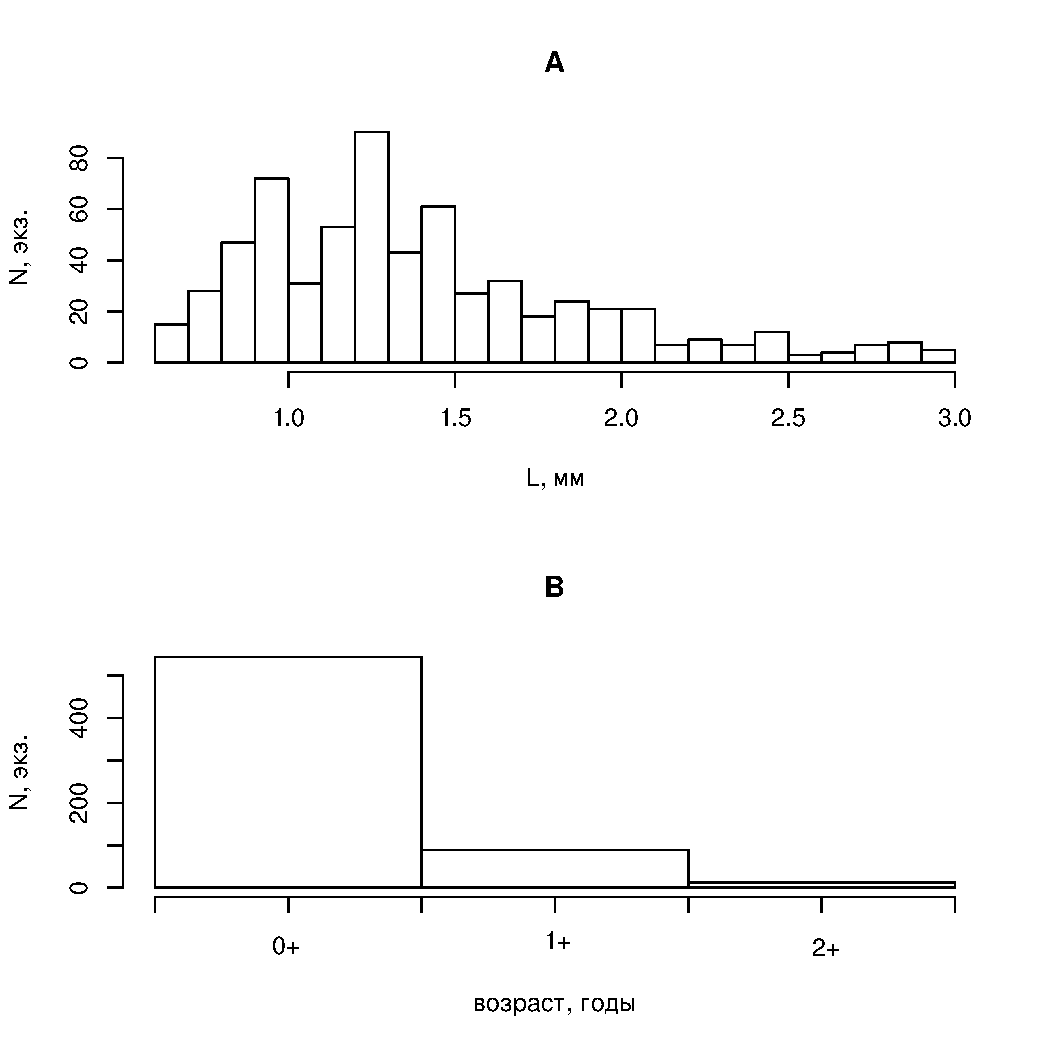
\includegraphics{../White_Sea/growth_young/hist_obili_po_godam1.pdf}
	\caption{Распределение моллюсков {\it M.~balthica} длиной менее $3$~см по размеру (А) и возрасту (В)}
	\label{ris:vozrast_menee_3mm}
	{\footnotesize Примечание: N, экз. \textemdash количество особей, L, мм \textemdash длина раковины}
	\end{figure}

Особи возрастом 1+ с различных горизонтов литорали острова Горелый не различаются по размеру ($Kruskal-Wallis\ \chi^2 = 3,12, p = 0,37$), поэтому в дальнейшем мы рассматриваем их как одну выборку (рис. \ref{ris:Goreliy_length1+_gorizonty}).
	\begin{figure}[hbp]
		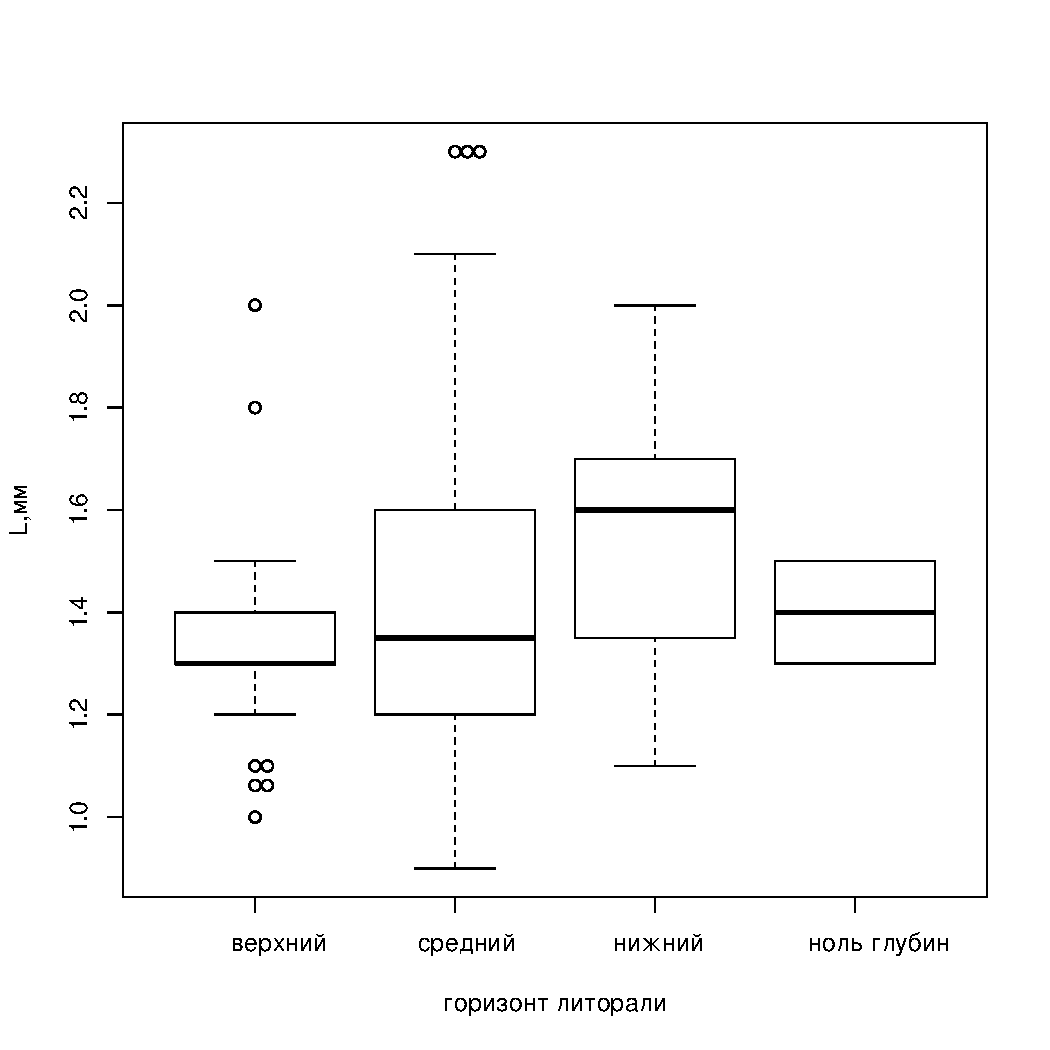
\includegraphics{../White_Sea/growth_young/boxplot_Goreliy_length_1+_tidal.pdf}
	\caption{Размеры  годовалых моллюсков {\it M.~balthica} на разных горизонтах литорали о. Горелый}
	\label{ris:Goreliy_length1+_gorizonty}
	{\footnotesize Примечание: L, мм \textemdash длина раковины. <<Ящик>> на графике соответствует 1 и 3 квартилю, жирная горизонтальная линия \textemdash 		медиана, <<усы>> \textemdash $1,5$ межквартильных размаха}
	\end{figure}

По результатам теста Краскел-Уоллиса годовалые моллюски с разных участков различались по длине ($Kruskal-Wallis\ \chi^2 = 17,6, p = 0,00015$) (\ref{ris:length_1+_uchastki}, поэтому было проведено попарное сравнение участков (табл.~\ref{tab:Tukey_1+_uchastki}). 
Размер годовалых особей не различался на участках, расположенных в районе Лувеньгиских шхер (о.~Горелый и эстуарий р.~Лувеньги), и отличался от особей из Западной Ряшковой салмы.
	\begin{figure}[hbp]
		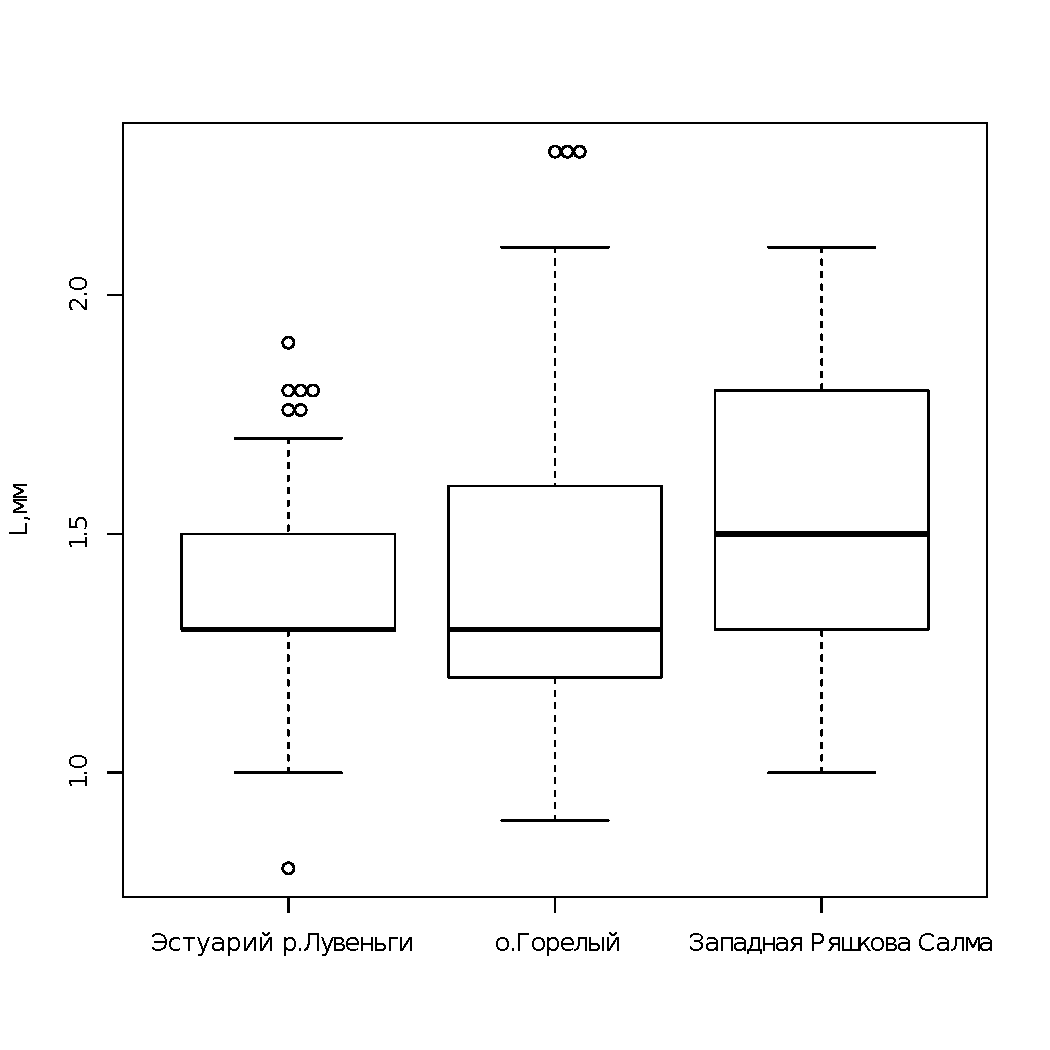
\includegraphics{../White_Sea/growth_young/boxplot_length_1age_area1.pdf}
	\caption{Размеры  годовалых моллюсков {\it M.~balthica} на разных участках литорали}
	\label{ris:length_1+_uchastki}
	{\footnotesize Примечание: L, мм \textemdash длина раковины. <<Ящик>> на графике соответствует 1 и 3 квартилю, жирная горизонтальная линия \textemdash 		медиана, <<усы>> \textemdash $1,5$ межквартильных размаха}
	\end{figure}
	
	\begin{table}[hbp]
	\caption{Результаты множественного сравнения длины годовалых {\it Macoma balthica} на различных участках методом Тьюки (Tukey's ‘Honest Significant Difference’).}
	\label{tab:Tukey_1+_uchastki}
	\begin{tabular}{|*{4}{p{0.2\textwidth}|}} \hline
	участки & различия средних & p-value & достоверность различий\\
	\hline
	о.~Горелый \textemdash\ эстуарий р.~Лувеньги & $0,053$ & $0,2$ & \\
	\hline
	о.~Горелый \textemdash\ Западная Ряшкова салма & $0,11$ & $0,005$ & ** \\
	\hline
	эстуарий р.~Лувеньги \textemdash\ Западная Ряшкова салма & $0,17$ & $0.00002$ & ***\\
	\hline
	\end{tabular}
	
	{\footnotesize Примечание: достоверность различий *** \textemdash $p<0,001$; ** \textemdash $p<0,05$; * \textemdash $p<0,1$.}
	\end{table}

Для определения границ размерно-возрастных классов {\it Macoma balthica} возрастом $0+$, $1+$ и $2+$ были рассчитаны средние размеры особей каждого возраста (табл~\ref{tab:mean_length_ages}).
	\begin{table}[hbp]	
\caption{Средний размер {\it Macoma balthica}в возрасте до 2 лет на различных участках.}
	\label{tab:mean_length_ages}
	\begin{tabular}{|l|*{3}{p{0.2\textwidth}|}} \hline
	возраст & $0+$ & $1+$ & $2+$\\
	\hline
	о.~Горелый & $1,0 \pm 0,001$ & $1,4 \pm 0,002$ & $2,2 \pm 0,008$ \\ 
	\hline
	эстуарий р.~Лувеньги & $1,0 \pm 0,004$ & $1,4 \pm 0,002$ & $2,2 \pm 0,02$ \\
	\hline
	Западная Ряшкова салма & $1,1 \pm 0,04$ & $1,5 \pm 0,003$ & $2,3 \pm 0,02$ \\ 
	\hline
	\end{tabular}
	
	{\footnotesize Примечание: В ячейках указано среднее арифметическое с ошибкой.}
	\end{table}
Пограничный размер между двумя когортами рассчитывали как середину между средними размерами особей в когорте. 
Таким образом, в дальнейшем для участков, расположенных в акватории Лувеньгских шхер, маком длиной менее $1,2$~мм рассматривали как спат, а длиной от $1,2$ до $1,8$~мм \textemdash\ как особей возрастом 1+.
Для участков на о.~Ряшков пограничные значения составили $1,3$ и $1,9$,~мм соответственно.
Для участка на о.Ломнишном мы использовали данные, полученные для о.~Ряшкова.

